% Options for packages loaded elsewhere
\PassOptionsToPackage{unicode}{hyperref}
\PassOptionsToPackage{hyphens}{url}
\PassOptionsToPackage{dvipsnames,svgnames,x11names}{xcolor}
%
\documentclass[
  onepage,
  openany]{scrbook}

\usepackage{amsmath,amssymb}
\usepackage{lmodern}
\usepackage{iftex}
\ifPDFTeX
  \usepackage[T1]{fontenc}
  \usepackage[utf8]{inputenc}
  \usepackage{textcomp} % provide euro and other symbols
\else % if luatex or xetex
  \usepackage{unicode-math}
  \defaultfontfeatures{Scale=MatchLowercase}
  \defaultfontfeatures[\rmfamily]{Ligatures=TeX,Scale=1}
\fi
% Use upquote if available, for straight quotes in verbatim environments
\IfFileExists{upquote.sty}{\usepackage{upquote}}{}
\IfFileExists{microtype.sty}{% use microtype if available
  \usepackage[]{microtype}
  \UseMicrotypeSet[protrusion]{basicmath} % disable protrusion for tt fonts
}{}
\makeatletter
\@ifundefined{KOMAClassName}{% if non-KOMA class
  \IfFileExists{parskip.sty}{%
    \usepackage{parskip}
  }{% else
    \setlength{\parindent}{0pt}
    \setlength{\parskip}{6pt plus 2pt minus 1pt}}
}{% if KOMA class
  \KOMAoptions{parskip=half}}
\makeatother
\usepackage{xcolor}
\usepackage[normalem]{ulem}
\setlength{\emergencystretch}{3em} % prevent overfull lines
\setcounter{secnumdepth}{5}
% Make \paragraph and \subparagraph free-standing
\ifx\paragraph\undefined\else
  \let\oldparagraph\paragraph
  \renewcommand{\paragraph}[1]{\oldparagraph{#1}\mbox{}}
\fi
\ifx\subparagraph\undefined\else
  \let\oldsubparagraph\subparagraph
  \renewcommand{\subparagraph}[1]{\oldsubparagraph{#1}\mbox{}}
\fi

\usepackage{color}
\usepackage{fancyvrb}
\newcommand{\VerbBar}{|}
\newcommand{\VERB}{\Verb[commandchars=\\\{\}]}
\DefineVerbatimEnvironment{Highlighting}{Verbatim}{commandchars=\\\{\}}
% Add ',fontsize=\small' for more characters per line
\newenvironment{Shaded}{}{}
\newcommand{\AlertTok}[1]{\textcolor[rgb]{1.00,0.00,0.00}{\textbf{#1}}}
\newcommand{\AnnotationTok}[1]{\textcolor[rgb]{0.38,0.63,0.69}{\textbf{\textit{#1}}}}
\newcommand{\AttributeTok}[1]{\textcolor[rgb]{0.49,0.56,0.16}{#1}}
\newcommand{\BaseNTok}[1]{\textcolor[rgb]{0.25,0.63,0.44}{#1}}
\newcommand{\BuiltInTok}[1]{#1}
\newcommand{\CharTok}[1]{\textcolor[rgb]{0.25,0.44,0.63}{#1}}
\newcommand{\CommentTok}[1]{\textcolor[rgb]{0.38,0.63,0.69}{\textit{#1}}}
\newcommand{\CommentVarTok}[1]{\textcolor[rgb]{0.38,0.63,0.69}{\textbf{\textit{#1}}}}
\newcommand{\ConstantTok}[1]{\textcolor[rgb]{0.53,0.00,0.00}{#1}}
\newcommand{\ControlFlowTok}[1]{\textcolor[rgb]{0.00,0.44,0.13}{\textbf{#1}}}
\newcommand{\DataTypeTok}[1]{\textcolor[rgb]{0.56,0.13,0.00}{#1}}
\newcommand{\DecValTok}[1]{\textcolor[rgb]{0.25,0.63,0.44}{#1}}
\newcommand{\DocumentationTok}[1]{\textcolor[rgb]{0.73,0.13,0.13}{\textit{#1}}}
\newcommand{\ErrorTok}[1]{\textcolor[rgb]{1.00,0.00,0.00}{\textbf{#1}}}
\newcommand{\ExtensionTok}[1]{#1}
\newcommand{\FloatTok}[1]{\textcolor[rgb]{0.25,0.63,0.44}{#1}}
\newcommand{\FunctionTok}[1]{\textcolor[rgb]{0.02,0.16,0.49}{#1}}
\newcommand{\ImportTok}[1]{#1}
\newcommand{\InformationTok}[1]{\textcolor[rgb]{0.38,0.63,0.69}{\textbf{\textit{#1}}}}
\newcommand{\KeywordTok}[1]{\textcolor[rgb]{0.00,0.44,0.13}{\textbf{#1}}}
\newcommand{\NormalTok}[1]{#1}
\newcommand{\OperatorTok}[1]{\textcolor[rgb]{0.40,0.40,0.40}{#1}}
\newcommand{\OtherTok}[1]{\textcolor[rgb]{0.00,0.44,0.13}{#1}}
\newcommand{\PreprocessorTok}[1]{\textcolor[rgb]{0.74,0.48,0.00}{#1}}
\newcommand{\RegionMarkerTok}[1]{#1}
\newcommand{\SpecialCharTok}[1]{\textcolor[rgb]{0.25,0.44,0.63}{#1}}
\newcommand{\SpecialStringTok}[1]{\textcolor[rgb]{0.73,0.40,0.53}{#1}}
\newcommand{\StringTok}[1]{\textcolor[rgb]{0.25,0.44,0.63}{#1}}
\newcommand{\VariableTok}[1]{\textcolor[rgb]{0.10,0.09,0.49}{#1}}
\newcommand{\VerbatimStringTok}[1]{\textcolor[rgb]{0.25,0.44,0.63}{#1}}
\newcommand{\WarningTok}[1]{\textcolor[rgb]{0.38,0.63,0.69}{\textbf{\textit{#1}}}}

\providecommand{\tightlist}{%
  \setlength{\itemsep}{0pt}\setlength{\parskip}{0pt}}\usepackage{longtable,booktabs,array}
\usepackage{calc} % for calculating minipage widths
% Correct order of tables after \paragraph or \subparagraph
\usepackage{etoolbox}
\makeatletter
\patchcmd\longtable{\par}{\if@noskipsec\mbox{}\fi\par}{}{}
\makeatother
% Allow footnotes in longtable head/foot
\IfFileExists{footnotehyper.sty}{\usepackage{footnotehyper}}{\usepackage{footnote}}
\makesavenoteenv{longtable}
\usepackage{graphicx}
\makeatletter
\def\maxwidth{\ifdim\Gin@nat@width>\linewidth\linewidth\else\Gin@nat@width\fi}
\def\maxheight{\ifdim\Gin@nat@height>\textheight\textheight\else\Gin@nat@height\fi}
\makeatother
% Scale images if necessary, so that they will not overflow the page
% margins by default, and it is still possible to overwrite the defaults
% using explicit options in \includegraphics[width, height, ...]{}
\setkeys{Gin}{width=\maxwidth,height=\maxheight,keepaspectratio}
% Set default figure placement to htbp
\makeatletter
\def\fps@figure{htbp}
\makeatother
\newlength{\cslhangindent}
\setlength{\cslhangindent}{1.5em}
\newlength{\csllabelwidth}
\setlength{\csllabelwidth}{3em}
\newlength{\cslentryspacingunit} % times entry-spacing
\setlength{\cslentryspacingunit}{\parskip}
\newenvironment{CSLReferences}[2] % #1 hanging-ident, #2 entry spacing
 {% don't indent paragraphs
  \setlength{\parindent}{0pt}
  % turn on hanging indent if param 1 is 1
  \ifodd #1
  \let\oldpar\par
  \def\par{\hangindent=\cslhangindent\oldpar}
  \fi
  % set entry spacing
  \setlength{\parskip}{#2\cslentryspacingunit}
 }%
 {}
\usepackage{calc}
\newcommand{\CSLBlock}[1]{#1\hfill\break}
\newcommand{\CSLLeftMargin}[1]{\parbox[t]{\csllabelwidth}{#1}}
\newcommand{\CSLRightInline}[1]{\parbox[t]{\linewidth - \csllabelwidth}{#1}\break}
\newcommand{\CSLIndent}[1]{\hspace{\cslhangindent}#1}

\usepackage{booktabs}
\usepackage{longtable}
\usepackage{array}
\usepackage{multirow}
\usepackage{wrapfig}
\usepackage{float}
\usepackage{colortbl}
\usepackage{pdflscape}
\usepackage{tabu}
\usepackage{threeparttable}
\usepackage{threeparttablex}
\usepackage[normalem]{ulem}
\usepackage{makecell}
\usepackage{xcolor}
\makeatletter
\makeatother
\makeatletter
\makeatother
\makeatletter
\@ifpackageloaded{caption}{}{\usepackage{caption}}
\AtBeginDocument{%
\ifdefined\contentsname
  \renewcommand*\contentsname{Table of contents}
\else
  \newcommand\contentsname{Table of contents}
\fi
\ifdefined\listfigurename
  \renewcommand*\listfigurename{List of Figures}
\else
  \newcommand\listfigurename{List of Figures}
\fi
\ifdefined\listtablename
  \renewcommand*\listtablename{List of Tables}
\else
  \newcommand\listtablename{List of Tables}
\fi
\ifdefined\figurename
  \renewcommand*\figurename{Figure}
\else
  \newcommand\figurename{Figure}
\fi
\ifdefined\tablename
  \renewcommand*\tablename{Table}
\else
  \newcommand\tablename{Table}
\fi
}
\@ifpackageloaded{float}{}{\usepackage{float}}
\floatstyle{ruled}
\@ifundefined{c@chapter}{\newfloat{codelisting}{h}{lop}}{\newfloat{codelisting}{h}{lop}[chapter]}
\floatname{codelisting}{Listing}
\newcommand*\listoflistings{\listof{codelisting}{List of Listings}}
\makeatother
\makeatletter
\@ifpackageloaded{caption}{}{\usepackage{caption}}
\@ifpackageloaded{subcaption}{}{\usepackage{subcaption}}
\makeatother
\makeatletter
\@ifpackageloaded{tcolorbox}{}{\usepackage[many]{tcolorbox}}
\makeatother
\makeatletter
\@ifundefined{shadecolor}{\definecolor{shadecolor}{named}{lightgray}}
\makeatother
\makeatletter
\@ifpackageloaded{sidenotes}{}{\usepackage{sidenotes}}
\@ifpackageloaded{marginnote}{}{\usepackage{marginnote}}
\makeatother
\makeatletter
\makeatother
\ifLuaTeX
  \usepackage{selnolig}  % disable illegal ligatures
\fi
\IfFileExists{bookmark.sty}{\usepackage{bookmark}}{\usepackage{hyperref}}
\IfFileExists{xurl.sty}{\usepackage{xurl}}{} % add URL line breaks if available
\urlstyle{same} % disable monospaced font for URLs
\hypersetup{
  pdftitle={THE VARAIBILITY CLIMATE CHANGE IS FESPONSIBLE FOR IN VEGETATION LOSS IN GHANA},
  pdfauthor={name:Kalong Boniface; Fugah Seletey Mitchell},
  colorlinks=true,
  linkcolor={Maroon},
  filecolor={Maroon},
  citecolor={blue},
  urlcolor={Blue},
  pdfcreator={LaTeX via pandoc}}

\title{THE VARAIBILITY CLIMATE CHANGE IS FESPONSIBLE FOR IN VEGETATION
LOSS IN GHANA}
\usepackage{etoolbox}
\makeatletter
\providecommand{\subtitle}[1]{% add subtitle to \maketitle
  \apptocmd{\@title}{\par {\large #1 \par}}{}{}
}
\makeatother
\subtitle{Quantifying The Status of Galamsey With Time Series Analsis}
\author{name:Kalong Boniface \and Fugah Seletey Mitchell}
\date{\texttt{r\ Sys.Date()}}

\begin{document}
\frontmatter
\maketitle
\begin{abstract}
\texttt{r\ paste(readLines("front-and-back-matter/\_abstract.qmd"),\ collapse\ =\ "\textbackslash{}n\ \ ")}
\end{abstract}
\ifdefined\Shaded\renewenvironment{Shaded}{\begin{tcolorbox}[boxrule=0pt, breakable, colback={shadecolor}, enhanced, frame hidden]}{\end{tcolorbox}}\fi

\renewcommand*\contentsname{Table of Contents}
{
\hypersetup{linkcolor=}
\setcounter{tocdepth}{2}
\tableofcontents
}
\listoffigures
\listoftables
\mainmatter
\hypertarget{chapter-one}{%
\chapter{CHAPTER ONE}\label{chapter-one}}

\hypertarget{introduction}{%
\section{INTRODUCTION}\label{introduction}}

One would anticipate that the majority of emerging nations, which are
still in the early stages of economic development and growth, would have
a high forest cover and little deforestation. This, however, has not
been the case. Ghana is a lower-middle-income nation that is still
working toward middle-income classification. However, it has already
begun to see a deforestation rate that is comparable to that of
middle-income countries. The rapid population expansion, clearing of
feild for Galamsey operation,increased domestic need for wood for things
like fuel, furniture, construction, and timber exports have all
contributed to this trend, Bush fires in the 1980s, climate change, and
lax law enforcement have all had an impact.

The purpose of this paper is to establish an understanding in time
series analysis on remotely sensed data. Which will introduced us to the
fundamentals of time series modeling, including decomposition,
autocorrelation and modeling historical changes in \textbf{Vegetation
Loss} in Ghana as a result of \textbf{Galamsey Operation} and the
\textbf{Variability Climate Is Responsible For}, the Cause, Dangers and
it's Environmental impact.

Galamsey also known as ``\emph{gather them and sell}'',Owusu-Nimo et al.
(\protect\hyperlink{ref-owusu-nimo2018}{2018}) is the term given by
local Ghanaian for illegal small-scale gold mining in Ghana . The major
cause of Galamsey is unemployment among the youth in Ghana Gracia
(\protect\hyperlink{ref-gracia2018}{2018}) . Young university graduates
rarely find work and when they do it hardly sustains them. The result is
that these youth go the extra mile to earn a living for themselves and
their family.

Another factor is that lack of job security. On November 13, 2009 a
collapse occurred in an illegal, privately owned mine in Dompoase, in
the Ashanti Region of Ghana. At least 18 workers were killed, including
13 women, who worked as porters for the miners. Officials described the
disaster as the worst mine collapse in Ghanaian history {``Women Die in
Ghana Mine Collapse''} (\protect\hyperlink{ref-womendi2009}{2009}) .

Illegal mining causes damage to the land and water supplym (Ansah
(\protect\hyperlink{ref-ansah2017}{2017}) ) . In March 2017, the
Minister of Lands and Natural Resources, Mr. John Peter Amewu, gave the
Galamsey operators/illegal miners a three-week ultimatum to stop their
activities or be prepared to face the law Allotey
(\protect\hyperlink{ref-allotey2017}{2017}) . The activities by
Galamseyers have depleted Ghana's forest cover and they have caused
water pollution, due to the crude and unregulated nature of the mining
process Gyekye (\protect\hyperlink{ref-gyekye}{n.d.}) .

Under current Ghanaian constitution, it is illegal to operate as
galamseyer.That is to dig on land granted to mining companies as
concessions or licenses and any other land in search for gold. In some
cases, Galamseyers are the first to discover and work extensive gold
deposits before mining companies find out and take over. Galamseyers are
the main indicator of the presence of gold in free metallic dust form or
they process oxide or sulfide gold ore using liquid mercury.

Between 20,000 to 50,000, including thousands from China are believed to
be engaged in Galamsey in Ghana.But according to the Information
Minister 200,000 and nearly 3 million people, recently are now into
Galamsey operation and rely on it for their livelihoods {``Gold, Guns
and China: Ghana's Fight to End Galamsey''}
(\protect\hyperlink{ref-goldgu2017}{2017}) . Their operations are mostly
in the southern part of Ghana where it is believe to have substantial
reserves of gold deposits, usually within the area of large mining
companies Barenblitt et al.
(\protect\hyperlink{ref-barenblitt2021}{2021}) . As a group, they are
economically disadvantaged. Galamsey settlements are usually poorer than
neighboring agricultural villages. They have high rates of accidents and
are exposed to mercury poisoning from their crude processing methods.
Many women are among the workers, acting mostly as porters for the
miners.

\hypertarget{background-of-the-study}{%
\subsection{Background of The Study}\label{background-of-the-study}}

As Galamsey is considered an illegal activity, they operations are
hidden to the eyes of the authorities.So locating them is quite tricky
,but with satellite imagery ,it now possible to locate their operating
and put an end to it. One of the features of Google Earth Engine is the
ability to access years of satellite imagery without needing to
download, organize, store and process this information. For instance,
within the Satellite image collection, now it possible to access imagery
back to the 90's, allowing us to look at areas of interest on the map to
visualize and quantify how much things has changed over time. With Earth
Engine, Google maintains the data and offers it's computing power for
processing.Users can now access hundreds of time series images and
analyze changes across decades using GIS and R or other programming
language to analyze these dataset.

\hypertarget{problem-statement}{%
\subsection{Problem Statement}\label{problem-statement}}

The Footprint of Galamsey is Spreading at a very faster rate, causing
vegetation loss.Other factors accounting to vegetation loss may largely
include climate change,urban and exurban development, bush fires. But
not much works or research has been done to tell the extent to which
Galamsey causes vegetation loss and the \textbf{Variability Climate
Change Is Responsible For}. This research attempts to segregate the
variability climate is responsible for in vegetation loss so as to
attribute the residual variability to Galamsey and other related
activities such as bush-fires etc.

\hypertarget{research-questions}{%
\subsection{Research Questions}\label{research-questions}}

To address the challenge of the vegetation variability in this work, the
following several statements were formed:

\begin{itemize}
\item
  Are there any changes in vegetation cause by Galamsey and Climate
  change in Ghana?
\item
  Is there any relationship between vegetation and land surface
  temperature in Ghana?
\end{itemize}

\hypertarget{research-objectives}{%
\subsection{Research Objectives}\label{research-objectives}}

The purpose is to establish an understanding in time series analysis on
remotely sensed data. We will be introduced to the fundamentals of time
series modeling, including decomposition, autocorrelation and modeling
historical changes.

\begin{itemize}
\item
  Perform time series analysis on satellite derived vegetation indices
\item
  Estimate the extent to which Galamsey causes vegetation loss in Ghana.
\item
  Dissociate or single out the variability climate is responsible for in
  vegetation loss
\end{itemize}

\hypertarget{significance-of-the-study}{%
\subsection{Significance Of The Study}\label{significance-of-the-study}}

There have been significant changes in vegetation cover in Ghana over
the past 30 years, and these dynamics are related strongly to climatic
factors such as temperature and other factors. In this study, we want to
examine the effects of climatic change on Ghana's vegetation during
these thirty years.

This study allows us to explore climatic differences and climate-related
drivers. Additionally, it offers a chance to research how climatic
variability affects the ecosystem and human health. By merging climate
and vegetation variation utilizing NDVI, LST, and EVI data to understand
the relationship between vegetation and climate change under tropical
climate conditions, it closes research gaps in Ghana. This study
explores historical and projected vegetation and climate data, by
sector, impacts, key vulnerabilities and what adaptation measures can be
taken. It also explores the overview for a general context of how
climate change is affecting \textbf{Ghana.}

\hypertarget{scope-of-the-study}{%
\subsection{Scope of The Study}\label{scope-of-the-study}}

\hypertarget{limitation-of-the-study}{%
\subsection{Limitation Of The Study}\label{limitation-of-the-study}}

The goal of time series modeling is to employ the simplest model
feasible to account for as much data as possible while still developing
an explanatory model of the data that does not over-fit the issue set.

Remote sensing data has additional limits that make this more difficult
when dividing time series data into component pieces. It is almost
certain that data from distant sensing will not provide the same level
of precision.

Additionally, atmospheric factors can distort the visual findings,
causing the vegetation's color to shift dramatically from image to image
as a result of atmospheric factors (fog, ground moisture, cloud cover).

\hypertarget{organization-of-the-study}{%
\subsection{Organization of The Study}\label{organization-of-the-study}}

\hypertarget{chapter-two}{%
\chapter{CHAPTER TWO}\label{chapter-two}}

\hypertarget{literature-review}{%
\section{LITERATURE REVIEW}\label{literature-review}}

The distribution of plant species, the richness and composition of plant
communities, the structure of the vegetation (such as biomass and leaf
area), and how the ecosystem uses water, nutrients, and carbon are all
predicted to change as a result of climate change. These plant responses
to climate change will be the outcome of numerous lower-level plant
reactions, such as adjustments in net plant carbon uptake, adjustments
in plant water usage, adjustments in plant growth and biomass
allocation, competitive interactions, and reactions to disturbances. It
is challenging to predict prospective plant reactions to future climatic
changes based only on theory or on laboratory and field studies due to
the complexity of climatic impacts on vegetation and the length of time
it takes for the responses to become obvious.

To project vegetation responses to changing climates, computer
simulation models that integrate theory and experimental results are
frequently used, and the following are some studies that have been done
previously where we reclassifies the drivers into human activity, and
climate change for an empirical review and None Parametric Test followed
by Time Series Analysis for the theoretical review .

\hypertarget{empirical-review}{%
\subsection{Empirical Review}\label{empirical-review}}

According to studies, there is now significant change in vegetation on
the earth than there was thirty years ago, and it is distributed
differently.

More than half of the changes they found are attributed to the
consequences of a warmer climate, with people only being responsible for
about a third. Perhaps surprisingly, they are unable to definitively
link approximately 10\% of the changes to either the climate or
us.@alex2013

Several models and hypotheses have been established in the environmental
literature to explain the relationship between human behaviour, and
environmental (forest) deforestation or depletion. Recent environmental
and energy economics literature focuses on the energy consumption
choices made by businesses and people in developing countries Gertler et
al. (\protect\hyperlink{ref-gertler2016}{2016}) . Africa's energy supply
is made mainly of fuel wood and charcoal to a degree of about 58\%.
Specht et al. (\protect\hyperlink{ref-specht2015}{2015}) . Before other
demands for forest goods like furniture and paper, the need for fuel
wood for cooking and heating is frequently identified as the main driver
of deforestation.

The causes of tropical forest decline are unclear, according to DeFries
et al. (\protect\hyperlink{ref-defries2010}{2010}) . However, scientists
were able to pinpoint the two primary causes of deforestation in the
21st century using information from satellite-based estimations in 41
different countries. The authors found a favorable association between
forest loss and increases in urban population as well as agricultural
exports using two methods of regression analysis. The same proof,
however, was not discovered in the case of the increase in rural
population. This suggests that forest loss is unavoidable in regions
with high levels of human activity.

\hypertarget{theoretical-review}{%
\subsection{Theoretical Review}\label{theoretical-review}}

This study review, will follow narrative approach to gain insight into
research topics. A time series is a set of observations, each being
recorded at a particular time and the collection of such observation is
referred to as time series data. The data is analysed to extract
statistical information, characteristics of the data and to predict the
output. As the data might tend to follow a pattern in time series data,
the Machine Learning model finds it difficult to predict appropriately
hence time series analysis and its approaches have made it simpler for
prediction.

\hypertarget{what-is-time-series-analysis}{%
\subsubsection{What is Time Series
Analysis?}\label{what-is-time-series-analysis}}

A time series in mathematics is a collection of data points that have
been listed, graphed, or indexed according to time. is a series of
photos taken at successive, evenly spaced intervals of time. Time series
are utilized in many areas of applied research that use temporal data,
including statistics, signal processing, pattern identification,
econometrics, mathematical finance, weather forecasting, and earthquake
prediction. Time series analysis refers to techniques for deriving
useful statistics and other aspects of time series data through
analysis. Time series forecasting is the process of using a model to
forecast future values based on values that have already been observed.
Regression analysis is frequently used to assess correlations between
one or more different time series, however this method of analysis is
not without its limitations.

In 1987 {``Confidence Intervals: An Empirical Investigation of the
Series in the m-Competition - ScienceDirect''}
(\protect\hyperlink{ref-confiden}{n.d.}) , Makridakis and Hibon, time
series analysis experts, held the M-Competition, where participants may
submit their forecasts on 1001 time series data drawn from economics,
industry, and demographics. The competition revealed four key findings,
including:

\begin{itemize}
\item
  Statistically sophisticated or complex methods do not necessarily
  provide more accurate forecasts than simpler ones.
\item
  The relative ranking of the performance of the various methods varies
  according to the accuracy measure being used.
\item
  The accuracy when various methods are being combined outperformed, on
  average, the individual methods being combined and does very well in
  comparison to other methods.
\item
  The accuracy of the various methods depends upon the length of the
  forecasting horizon involved.
\end{itemize}

The time series data is visualized and analyzed to find out mainly three
things, trend, seasonality, and Heteroscedasticity.

\textbf{Trend:} It can be characterized as the observation of a rising
or escalating pattern throughout time. While in normal time series the
mean is an arbitrary function of time, in stationary time series the
mean of the data must be constant across time.

\textbf{Seasonality:} This term describes a cycle of events. a pattern
that, after some time, keeps happening.

\textbf{Heteroscedasticity:} It is also referred to as level, and it is
described as the non-constant variance from the mean computed over time.

Few approaches do not perform well when trends are present in the data,
and even fewer do not perform well when the data is seasonal. In order
to choose the optimal statistical method for forecasting, trends,
seasonality, and heteroscedasticity must be taken into account.

\hypertarget{time-series-forecasting-using-stochastic-models}{%
\subsubsection{\texorpdfstring{\textbf{Time Series Forecasting Using
Stochastic
Models}}{Time Series Forecasting Using Stochastic Models}}\label{time-series-forecasting-using-stochastic-models}}

The selection of a proper model is extremely important as it reflects
the underlying structure of the series and this fitted model in turn is
used for future forecasting. A time series model is said to be linear or
non-linear depending on whether the current value of the series is a
linear or non-linear function of past observations.

In general models for time series data can have many forms and represent
different stochastic processes. There are two widely used linear time
series models in literature.

\emph{Autoregressive (AR)} and \emph{Moving Average (MA)} models,
combining these two, the Autoregressive Moving Average (ARMA) and
\emph{Autoregressive Integrated Moving Average (ARIMA)} models have been
proposed in many literature. The \emph{Autoregressive Fractionally
Integrated Moving Average (ARFIMA)} model generalizes ARMA and ARIMA
models. For seasonal time series forecasting, a variation of ARIMA. The
\emph{Seasonal Autoregressive Integrated Moving Average (SARIMA)} {]}
model is used.

ARIMA model and its different variations are based on the famous
Box-Jenkins principle Hipel and McLeod
(\protect\hyperlink{ref-hipel1994}{1994}) and so these are also broadly
known as the Box-Jenkins models.

Linear models have drawn much attention due to their relative simplicity
in understanding and implementation. However many practical time series
show non-linear patterns. For example, as mentioned by R. Parrelli in ,
non-linear models are appropriate for predicting volatility changes in
economic and financial time series. Considering these facts, various
non-linear models have been suggested in literature. Some of them are
the famous Autoregressive Conditional Heteroskedasticity (ARCH) model
and its variations like Generalized ARCH (GARCH) , Exponential
Generalized ARCH (EGARCH) etc., the Threshold Autoregressive (TAR)
model, the Non-linear Autoregressive (NAR) model, the Non-linear Moving
Average (NMA) model, All the methods consider either of trend,
seasonality, or heteroscedasticity to predict the future output. Time
series data must be decomposed based on the findings from data analysis.
Based on the findings from analysis data must be broken into trend or
seasonality. Zhang, Eddy Patuwo, and Y. Hu
(\protect\hyperlink{ref-zhang1998}{1998})

\hypertarget{exponential-smoothing-models}{%
\paragraph{Exponential Smoothing
Models:}\label{exponential-smoothing-models}}

Time-series data relies on the assumption that the observation at a
certain point of time depends on previous observations in time . The
previous observations are given weights as they contribute to the future
prediction. The process of weighting is done using a notation called
`\textbf{Theta}'. To find the best possible value for theta, we must
perform sum of squared errors between the actual versus predicted value
of the previous observation. Using this process, we can predict the next
value but to predict more than one value this process does contribute
much as the prediction as going to be same as the previous value.

To understand the methods and to evaluate different models, few concepts
like \emph{stationarity} and \emph{differencing} must be understood.
Both these concepts help in making the core concepts of the methods easy
to interpret.

\hypertarget{stationarity}{%
\paragraph{\texorpdfstring{\textbf{Stationarity:}}{Stationarity:}}\label{stationarity}}

Stationarity alludes to an irregular process that creates a time-series
which has mean, and distribution to be constant through time.
Distribution only depends on time and not location in time (Manuca, R.
and Savit, R., 1996). If the distribution is same over different time
windows is strong stationarity and if only mean and variance are
similar, then it is weak stationarity. Irrespective of strong or weak,
stationarity helps build a class of models such Autoregression (AR),
Moving Average (MA), ARIMA (Witt, A., Kurths, J. and Pikovsky, A.,
1998).

An MA(q) process is always stationary, irrespective of the values the MA
parameters {[}23{]}. The conditions regarding stationarity and
invertibility of AR and MA processes also hold for an ARMA process. An
ARMA(p, q) process is stationary if all the roots of the characteristic
equation \(\phi (L) = 0\) lie outside the unit circle. Similarly, if all
the roots of the lag equation

\(\theta (L) = 0\) lie outside the unit circle, then the ARMA(p, q)
process is invertible and can be expressed as a pure AR process..

\hypertarget{differencing}{%
\paragraph{\texorpdfstring{\textbf{Differencing:}}{Differencing:}}\label{differencing}}

This concept is used to make trending and seasonal data stationary.
Subtraction between current observation and previous observation is the
process of differencing. It helps in making the mean constant (Dickey,
D.A. and Pantula, S.G., 1987).

\hypertarget{autoregressive-models-ar}{%
\paragraph{\texorpdfstring{\textbf{Autoregressive models
(AR):}}{Autoregressive models (AR):}}\label{autoregressive-models-ar}}

AR work on a concept called lags which is defined as the forecast of a
series is solely based on the past values in the series (Cryer, J.D.,
1986). Formula for Autoregression AR(1):
\(\displaystyle y_{t} = \omega + \phi Y _{t-1}+ e_{t}\) is stationary
when \$\textbar{}\phi\_\{1\}\textbar\textless{} 1\$ with a constant mean
\(\displaystyle \mu = \frac{\omega}{1-\phi_{1}}\) and constant variance
\(\displaystyle \gamma_{o} = \frac{\sigma^{2}}{1-\phi_{1}^{2}}\) Where ;
\(y_{t}\) = Target , \(\omega\) = Intercept, \(\phi\) = Coefficient,
\(Y_{t-1}\)=Lagged target, \(e_{t}\) = Error\textbackslash{}

It depends only on one lag in the past and also called AR model of order
one (Shibata, R., 1976). Autoregressive models are also known as long
memory models as they must keep the memory of all the lags until its
initial start point and must calculate their value. If there is any
shock incident in the past which must have led to fluctuations in the
data, it will have its effect on the present value which makes the model
quite sensitive to shocks (Shibata, R., 1976).

\hypertarget{moving-average-ma}{%
\paragraph{\texorpdfstring{\textbf{Moving Average
(MA):}}{Moving Average (MA):}}\label{moving-average-ma}}

The moving average model forecasts a series based on the past error in
the series called error lags. Hunter, J.S., Formula for moving average
method is given as: \(y_{t} = \omega + \theta e _{t-1}+ e_{t}\)

In (2), all the abbreviations are same to AR model formula except, =
Previous error

There arises a question as this method uses the error for the previous
value but when it reaches to the first point there will be no previous
value, to overcome this the average of the series is considered as the
value before the starting point. These are short memory models as the
error in the past will not have much effect on the future value (Hunter,
J.S., 1986).

\hypertarget{comparing-ar-method-with-ma-method}{%
\paragraph{\texorpdfstring{\textbf{Comparing AR method with MA
method:}}{Comparing AR method with MA method:}}\label{comparing-ar-method-with-ma-method}}

Let focus on the two methods which were used in the early years of time
series forecasting and compare the performance of each model on a
particular task. Testing against general autoregressive and moving
average error models where the regressors include lagged dependent
variables. (Godfrey, L.G., 1978) In their paper have explained the order
of the error process under the alternate hypothesis using lagrange
multiplier test (Silvey, S.D., 1959). As per the tests the errors of
both the models were similar, but the constraints were different under
which the tests were performed are also to be considered. As they have
concluded in their paper stating that that the outcome of the model's
performance depends on the estimate chosen to be null hypothesis or
alternate hypothesis.

In addition, paper written by (Baltagi, B.H. and Li, Q., 1995),
Demonstrates the comparison of AR and MA model using Burke, Godfrey, and
Termayne test. To the error component model. They explained choosing of
this test is because these are simple to implement as they only require
within residual or OLS residual (Baltagi, B.H. and Li, Q., 1995). The
outcome of the experiment was explained as when the test used within
residual AR model performed well but had problems, if the test used OLS
residual MA model performance was good. They have concluded stating that
MA will performance much better when the parameters are changed.

The findings of both the paper were quite different but one cannot prove
either of the model to be better as the performance depends on the
parameters used in the model. Each model is unique to its use case, and
it depends on the user to choose accordingly based on the data.

\hypertarget{autocorrelation-and-partial-autocorrelation-functions-acf-and-pacf}{%
\paragraph{\texorpdfstring{\textbf{Autocorrelation and Partial
Autocorrelation Functions (ACF and
PACF)}}{Autocorrelation and Partial Autocorrelation Functions (ACF and PACF)}}\label{autocorrelation-and-partial-autocorrelation-functions-acf-and-pacf}}

To determine a proper model for a given time series data, it is
necessary to carry out the ACF and PACF analysis. These statistical
measures reflect how the observations in a time series are related to
each other. For modeling and forecasting purpose it is often useful to
plot the ACF and PACF against consecutive time lags. These plots help in
determining the order of AR and MA terms. For a time series
\({x(t),t = 0,1, 2,...}\)the Autocovariance {[}21, 23{]} at lag k is
defined as:

\(\mu\) is the mean of the time series, i.e.
\(\mu = E\left[x_{t}\right]\). The autocovariance at lag zero i.e.
\(y_{0}\) is the variance of the time series. From the definition it is
clear that the autocorrelation coefficient \$ p\_\{k\}\$ is
dimensionless and so is independent of the scale of measurement. Also,
clearly \(-1 \leq p\_{k}\leq 1\). Statisticians Box and Jenkins {[}6{]}
termed \(y_{k }\) as the theoretical Autocovariance Function (ACVF) and
\(p_{k}\) as the theoretical Autocorrelation Function (ACF).

Another measure, known as the Partial Autucorrelation Function (PACF) is
used to measure the correlation between an observation k period ago and
the current observation, after controlling for observations at
intermediate lags (i.e. at lags \textless{} k ) {[}12{]}. At lag 1,
PACF(1) is same as ACF(1). The detailed formulae for calculating PACF
are given in {[}6, 23{]}.

Normally, the stochastic process governing a time series is unknown and
so it is not possible to determine the actual or theoretical ACF and
PACF values. Rather these values are to be estimated from the training
data, i.e. the known time series at hand. The estimated ACF and PACF
values from the training data are respectively termed as sample ACF and
PACF {[}6, 23{]}.

As given in {[}23{]}, the most appropriate sample estimate for the ACVF
at lag k is ACF plot is useful in determining the type of model to fit
to a time series of length N. Since ACF is symmetrical about lag zero,
it is only required to plot the sample ACF for positive lags, from lag
one on-wards to a maximum lag of about N/4. The sample PACF plot helps
in identifying the maximum order of an AR process.

\hypertarget{autoregressive-moving-average-arma-model}{%
\subsubsection{\texorpdfstring{\textbf{Autoregressive Moving Average
(ARMA)
model:}}{Autoregressive Moving Average (ARMA) model:}}\label{autoregressive-moving-average-arma-model}}

ARMA model is a combination of AR and MA models. The equation of the AR
model of order one, when it reaches to the starting point will have
infinite moving average (Choi, B., 2012). In ARMA model p and q have to
defined, where p = number of significant terms in ACF and q = number of
significant terms in PACF.

To determine the optimal value for p and q there are two ways:

\begin{itemize}
\item
  Plotting patterns in correlation
\item
  Automatic selection techniques
\end{itemize}

\hypertarget{plotting-patterns-in-correlation}{%
\paragraph{\texorpdfstring{\textbf{Plotting patterns in
correlation:}}{Plotting patterns in correlation:}}\label{plotting-patterns-in-correlation}}

\hypertarget{auto-correlation-factor-acf}{%
\subparagraph{\texorpdfstring{\textbf{Auto correlation factor
(ACF):}}{Auto correlation factor (ACF):}}\label{auto-correlation-factor-acf}}

It is the correlation between the observations at the current time stamp
and observations at the previous time stamp (Hagan, M.T. and Behr, S.M.,
1987).

\hypertarget{partial-auto-correlation-factor-pacf}{%
\subparagraph{\texorpdfstring{\textbf{Partial auto correlation factor
(PACF):}}{Partial auto correlation factor (PACF):}}\label{partial-auto-correlation-factor-pacf}}

The correlation between the observations at two different time stamps,
assuming both observations are correlated to the observations at another
time stamp (Hagan, M.T. and Behr, S.M., 1987).

\hypertarget{automatic-selection-techniques}{%
\paragraph{\texorpdfstring{\textbf{Automatic selection
techniques:}}{Automatic selection techniques:}}\label{automatic-selection-techniques}}

There are three commonly used techniques for automatic selection of time
series model:

\hypertarget{section}{%
\subparagraph{}\label{section}}

\begin{itemize}
\item
  \emph{Minimum info criteria (MINIC):}This builds multiple combinations
  of models across a grid search of AR and MA terms. It then finds the
  model with lowest Bayesian information criteria (Stadnytska, T.,
  Braun, S. and Werner, J., 2008).
\item
  \emph{Squared canonical correlations (SCAN):} It looks at correlation
  matrix of the data, then it compares it with its lags. It then looks
  at the eigen values from the correlation matrix to find the
  combination of AR and MA probably having SCAN as 0. It finds the pair
  as the best where the convergence is quickest (Stadnytska, T., Braun,
  S. and Werner, J., 2008).
\item
  \emph{The extended sample auto correlation function (ESACF):} As it is
  known that AR and MA are related. Essentially it filters out the AR
  terms until only MA piece is left. This process is repeated until
  fewest AR terms are left and maximum MA terms (Stadnytska, T., Braun,
  S. and Werner, J., 2008).

  It completely depends on the individual to choose from either of the
  methods helping them to find the optimal value of p and q for better
  performance of the model.
\end{itemize}

\hypertarget{autoregressive-integrated-moving-average-arima}{%
\subsubsection{\texorpdfstring{\textbf{Autoregressive Integrated Moving
average
(ARIMA):}}{Autoregressive Integrated Moving average (ARIMA):}}\label{autoregressive-integrated-moving-average-arima}}

To understand ARIMA model, we need to understand ARMA model as this is
just an extension to ARMA model. Essentially, we need to make data
stationary to feed it to a machine learning model. It is done by through
differencing. ARIMA models are mathematically written as
\textbf{\emph{ARIMA(p,d,q)}}, where p and q are same as ARMA model but
\textbf{\emph{d}} = number of first differences (Yu, G. and Zhang, C.,
2004, May).

\hypertarget{seasonal-autoregressive-integrated-moving-average-sarima}{%
\subsubsection{\texorpdfstring{\textbf{Seasonal Autoregressive
Integrated Moving Average
(SARIMA):}}{Seasonal Autoregressive Integrated Moving Average (SARIMA):}}\label{seasonal-autoregressive-integrated-moving-average-sarima}}

SARIMA models were introduced to handle seasonality in the data.
Seasonality is different from stationarity; however, seasonality can be
handled using stationarity up to some extent, but seasonal correlations
cannot be eliminated completely. SARIMA models are mathematically
written as SARIMA\((p,d,q)(P,D,Q)^{s}\).

Where;

P = Number of seasonal AR terms, D = Number of seasonal differences, Q =
Number of seasonal MA terms, s = Length of the season.

Removing seasonality will help the model to perform better but getting
rid of seasonality in data is a difficult task to do.

\hypertarget{comparing-arima-method-with-sarima-method}{%
\subsubsection{\texorpdfstring{\textbf{Comparing ARIMA method with
SARIMA
method:}}{Comparing ARIMA method with SARIMA method:}}\label{comparing-arima-method-with-sarima-method}}

Library and Valipour (\protect\hyperlink{ref-library2015}{2015})
investigated it on long-term runoff forecasting in the United States in
contrast to ARIMA and SARIMA. The outcomes demonstrated that SARIMA
models outperformed ARIMA models. However, it was discovered that SARIMA
models were extremely sensitive, and even a small change in a parameter
would have a negative impact on the model's performance. ARIMA and
SARIMA models have been applied by (Wang, S., Li, C., and Lim, 2019)
from the perspectives of Linear System Analysis, Spectra Analysis, and
Digital Filtering. The researchers were obliged to go outside of these
models for greater performance after it was established that ARIMA and
SARIMA both had poor performance.Although they claimed the ARMA-SIN
model was superior to the ARIMA and SARIMA models, they also
acknowledged that it was more challenging to study and comprehend the
ideas.

The results of Library and Valipour
(\protect\hyperlink{ref-library2015}{2015}) have demonstrated that
SARIMA is superior; however, their assertion is incongruent when it is
contrasted with the results of (Wang, S., Li, C. and Lim, A., 2019).

The choice of a particular approach must be based on the data; following
analysis, it is known whether the data have a trend, in which case ARIMA
must be used, or whether they are seasonal, in which case SARIMA would
be beneficial.

\hypertarget{advantages-and-disadvantages-of-time-series-forecasting}{%
\subsubsection{\texorpdfstring{\textsc{\textbf{ADVANTAGES AND
DISADVANTAGES OF TIME SERIES
FORECASTING}}}{ADVANTAGES AND DISADVANTAGES OF TIME SERIES FORECASTING}}\label{advantages-and-disadvantages-of-time-series-forecasting}}

\textbf{Advantages of time series forecasting:}

\begin{itemize}
\item
  Time series forecasting is of high accuracy and simplicity.
\item
  It can be used to analyze how the changes associated with the data
  point picked correlate with changes in other variables during the same
  time span.
\item
  Statistical techniques have been developed to analyze time series in
  such a way that the factor that influences the fluctuation of the
  series may be identified and handled.
\item
  It can give good output with less variables. As regression models fail
  with less variables, time series models will work better and
  effectively.
\end{itemize}

\textbf{Disadvantages of time series forecasting:}

\begin{itemize}
\item
  Time series models can easily be overfitted, which lead to false
  results.
\item
  It works well with short term forecasting but does not work well with
  long term forecasting.
\item
  It is sensible to outliers, if the outliers are not handled properly
  then it could lead to wrong predictions.
\item
  The different elements that impact the fluctuations of a series cannot
  be fully adjusted by the time series analysis
\end{itemize}

\hypertarget{forecast-performance-measures}{%
\subsubsection{Forecast Performance
Measures}\label{forecast-performance-measures}}

While applying a particular model to some real or simulated time series,
first the raw data is divided into two parts (\textbf{Training Set and
Test Set}). The observations in the training set are used for
constructing the desired model. Often a small sub-part of the training
set is kept for validation purpose and is known as the
\textbf{Validation Set}. Sometimes a preprocessing is done by
normalizing the data or taking logarithmic or other transforms. One such
famous technique is the Box-Cox Transformation {[}23{]}. Once a model is
constructed, it is used for generating forecasts. The test set
observations are kept for verifying how accurate the fitted model
performed in forecasting these values. If necessary, an inverse
transformation is applied on the forecast values to convert them in
original scale. In order to judge the forecasting accuracy of a
particular model or for evaluating and comparing different models, their
relative performance on the test dataset is considered.

Due to the fundamental importance of time series forecasting in many
practical situations, proper care should be taken while selecting a
particular model. For this reason, various performance measures are
proposed in literature {[}3, 7, 8, 9, 24, 27{]} to estimate forecast
accuracy and to compare different models. These are also known as
performance metrics {[}24{]}. Each of these measures is a function of
the actual and forecast values of the time series.

\hypertarget{description-of-various-forecast-performance-measures}{%
\paragraph{Description of Various Forecast Performance
Measures}\label{description-of-various-forecast-performance-measures}}

In each of the forthcoming definitions, \(y_{t }\) is the actual value,
\(f_{t}\) is the forecaste value, \(e_{t} = y_{t} - f_{t}\) is the
forecast error and n is the size of the test set. Also,
\(\displaystyle \bar{y} = \frac{1}{n}\sum_{t=1}^{n}y_{t}\) is the test
mean and
\(\displaystyle \sigma^{2} = \frac{1}{n-1}\sum_{t=1}^{n}(y_{t}-\bar{y})^{2}\)is
the test variance.

\hypertarget{the-mean-forecast-error-displaystyle-mfe-frac1nsum_t1ne_t}{%
\subparagraph{\texorpdfstring{\textbf{The Mean Forecast Error}
\(\displaystyle MFE = \frac{1}{n}\sum_{t=1}^{n}e_{t}\)}{The Mean Forecast Error \textbackslash displaystyle MFE = \textbackslash frac\{1\}\{n\}\textbackslash sum\_\{t=1\}\^{}\{n\}e\_\{t\}}}\label{the-mean-forecast-error-displaystyle-mfe-frac1nsum_t1ne_t}}

• It is a measure of the average deviation of forecasted values from
actual ones.

• It shows the direction of error and thus also termed as the Forecast
Bias.

• In MFE, the effects of positive and negative errors cancel out and
there is no way to

know their exact amount.

• A zero MFE does not mean that forecasts are perfect, i.e. contain no
error; rather it only

indicates that forecasts are on proper target.

• MFE does not panelize extreme errors.

• It depends on the scale of measurement and also affected by data
transformations.

• For a good forecast, i.e. to have a minimum bias, it is desirable that
the MFE is as close

to zero as possible.

\hypertarget{the-mean-absolute-error-displaystyle-mae-frac1nsum_t1ne_t}{%
\subparagraph{\texorpdfstring{The Mean Absolute Error
\(\displaystyle MAE = \frac{1}{n}\sum_{t=1}^{n}|e_{t}|\)}{The Mean Absolute Error \textbackslash displaystyle MAE = \textbackslash frac\{1\}\{n\}\textbackslash sum\_\{t=1\}\^{}\{n\}\textbar e\_\{t\}\textbar{}}}\label{the-mean-absolute-error-displaystyle-mae-frac1nsum_t1ne_t}}

\begin{itemize}
\tightlist
\item
  It measures the average absolute deviation of forecast values from
  original ones.
\end{itemize}

-It is also termed as the Mean Absolute Deviation (MAD).

\begin{itemize}
\item
  It shows the magnitude of overall error, occurred due to forecasting.
\item
  In MAE, the effects of positive and negative errors do not cancel out.
\item
  Unlike MFE, MAE does not provide any idea about the direction of
  errors.
\item
  For a good forecast, the obtained MAE should be as small as possible.
\item
  Like MFE, MAE also depends on the scale of measurement and data
  transformations.
\item
  Extreme forecast errors are not panelized by MAE.
\end{itemize}

\hypertarget{the-mean-squared-error-displaystyle-mse-frac1nsum_t1ne2_t}{%
\subparagraph{\texorpdfstring{The Mean Squared Error
\(\displaystyle MSE = \frac{1}{n}\sum_{t=1}^{n}e^{2}_{t}\)}{The Mean Squared Error \textbackslash displaystyle MSE = \textbackslash frac\{1\}\{n\}\textbackslash sum\_\{t=1\}\^{}\{n\}e\^{}\{2\}\_\{t\}}}\label{the-mean-squared-error-displaystyle-mse-frac1nsum_t1ne2_t}}

\begin{itemize}
\item
  It is a measure of average squared deviation of forecast values.
\item
  As here the opposite signed errors do not offset one another, MSE
  gives an overall idea of the error occurred during forecasting.
\item
  It panelizes extreme errors occurred while forecasting.
\item
  MSE emphasizes the fact that the total forecast error is in fact much
  affected by large
\item
  individual errors, i.e. large errors are much expensive than small
  errors.
\item
  MSE does not provide any idea about the direction of overall error.
\item
  MSE is sensitive to the change of scale and data transformations.
\item
  Although MSE is a good measure of overall forecast error, but it is
  not as intuitive and
\item
  easily interpretable as the other measures discussed before.

  \hypertarget{the-root-mean-squared-error-displaystyle-rmse-sqrtmse-sqrt-frac1nsum_t1ne2_t}{%
  \subparagraph{\texorpdfstring{The Root Mean Squared Error
  \(\displaystyle RMSE = \sqrt{MSE} = \sqrt {\frac{1}{n}\sum_{t=1}^{n}e^{2}_{t}}\)}{The Root Mean Squared Error \textbackslash displaystyle RMSE = \textbackslash sqrt\{MSE\} = \textbackslash sqrt \{\textbackslash frac\{1\}\{n\}\textbackslash sum\_\{t=1\}\^{}\{n\}e\^{}\{2\}\_\{t\}\}}}\label{the-root-mean-squared-error-displaystyle-rmse-sqrtmse-sqrt-frac1nsum_t1ne2_t}}

  RMSE is nothing but the square root of calculated MSE.

  All the properties of MSE hold for RMSE as well.
\end{itemize}

\hypertarget{chapter-three}{%
\chapter{CHAPTER THREE}\label{chapter-three}}

\hypertarget{methodology}{%
\section{METHODOLOGY}\label{methodology}}

Data from a time series is a set of observations made in a particular
order over a period of time. There is a chance for correlation between
observations because time series data points are gathered at close
intervals. To help machine learning classifiers work with time series
data, we provide several new tools. We first contend that local features
or patterns in time series can be found and combined to address
challenges involving time-series categorization. Then, a method to
discover patterns that are helpful for classification is suggested. We
combine these patterns to create computable categorization rules. In
order to mask low-quality pixels, we will first collect data from Google
Earth Engine in order to choose NDVI, EVI values and Climate Change
data.

Instead of analyzing the imagery directly, we will summarize the mean
NDVI and EVI values. This will shorten the analysis time while still
providing an attractive and useful map. We will apply a smoothing
strategy using an ARIMA function to fix the situation where some cells
may not have NDVI and EVI for a particular month. Once NA values have
been eliminated, the time series will be divided to eliminate
seasonality before the normalized data is fitted using a linear model.
We will go to classify our data on the map and map it after we have
extracted the linear trend.

\hypertarget{research-design}{%
\section{Research Design}\label{research-design}}

In this study, the submission used a quantitative approach. Instead of
using subjective judgment, findings and conclusions heavily rely on the
use of statistical methods and reliable time series models.

\hypertarget{data-representation}{%
\subsection{Data Representation}\label{data-representation}}

The Republic of Ghana, a nation in West Africa, will serve as the
location for the experimental plots for this study. It shares borders
with the Ivory Coast in the west, Burkina Faso in the north, and Togo in
the east. It borders the Gulf of Guinea and the Atlantic Ocean to the
south. Ghana's total size is 238,535 km2 (92,099 sq mi), and it is made
up of a variety of biomes, from tropical rainforests to coastal
savannas. Ghana, which has a population of over 31 million, is the
second-most populous nation in West Africa, behind Nigeria.Accra, the
nation's capital and largest city, as well as Kumasi, Tamale, and
Sekondi-Takoradi, are other important cities.

\hypertarget{assumptions}{%
\subsection{Assumptions}\label{assumptions}}

\begin{Shaded}
\begin{Highlighting}[]
\CommentTok{\# | label: tbl{-}Data Frame}
\CommentTok{\# | tbl{-}cap: "Collected from Google Earth Engine"}
\NormalTok{Data\_Frame }\OtherTok{\textless{}{-}} \FunctionTok{read.csv}\NormalTok{(}\StringTok{"Data/Time\_Series.csv"}\NormalTok{)}
\NormalTok{Time\_Serie }\OtherTok{\textless{}{-}} \FunctionTok{read.csv}\NormalTok{(}\StringTok{"Data/Time\_Series.csv"}\NormalTok{)}\SpecialCharTok{\%\textgreater{}\%}
  \FunctionTok{select}\NormalTok{(year,NDVI,EVI,Precipitation,MinTemperature,MaxTemperature)}\SpecialCharTok{\%\textgreater{}\%}
  \FunctionTok{group\_by}\NormalTok{(year)}\SpecialCharTok{\%\textgreater{}\%}
  \FunctionTok{summarise\_each}\NormalTok{(}\FunctionTok{funs}\NormalTok{(median))}

\FunctionTok{kable}\NormalTok{(Time\_Serie,}\AttributeTok{longtable =}\NormalTok{ T, }\AttributeTok{booktabs =}\NormalTok{ T)}\SpecialCharTok{\%\textgreater{}\%}
\FunctionTok{add\_header\_above}\NormalTok{(}\FunctionTok{c}\NormalTok{(}\StringTok{" "}\NormalTok{,}\StringTok{"Vegetation Indices"} \OtherTok{=} \DecValTok{2}\NormalTok{,}\StringTok{"Climate Change"}\OtherTok{=} \DecValTok{3}\NormalTok{))}\SpecialCharTok{\%\textgreater{}\%}
  \FunctionTok{kable\_styling}\NormalTok{(}\AttributeTok{latex\_options =} \FunctionTok{c}\NormalTok{(}\StringTok{"repeat\_header"}\NormalTok{))}
\end{Highlighting}
\end{Shaded}

\begin{longtable}{rrrrrr}
\toprule
\multicolumn{1}{c}{ } & \multicolumn{2}{c}{Vegetation Indices} & \multicolumn{3}{c}{Climate Change} \\
\cmidrule(l{3pt}r{3pt}){2-3} \cmidrule(l{3pt}r{3pt}){4-6}
year & NDVI & EVI & Precipitation & MinTemperature & MaxTemperature\\
\midrule
\endfirsthead
\multicolumn{6}{@{}l}{\textit{(continued)}}\\
\toprule
\multicolumn{1}{c}{ } & \multicolumn{2}{c}{Vegetation Indices} & \multicolumn{3}{c}{Climate Change} \\
\cmidrule(l{3pt}r{3pt}){2-3} \cmidrule(l{3pt}r{3pt}){4-6}
year & NDVI & EVI & Precipitation & MinTemperature & MaxTemperature\\
\midrule
\endhead

\endfoot
\bottomrule
\endlastfoot
2001 & 0.7499792 & 0.5585050 & 92.40138 & 217.8009 & 339.8688\\
2002 & 0.6174545 & 0.4369971 & 128.81453 & 218.3945 & 335.7865\\
2003 & 0.6536485 & 0.4331280 & 126.15505 & 220.3344 & 335.7901\\
2004 & 0.8261204 & 0.5229186 & 111.66388 & 218.4170 & 330.1023\\
2005 & 0.7293837 & 0.4568775 & 97.24309 & 221.1652 & 331.5585\\
\addlinespace
2006 & 0.7049664 & 0.4158985 & 94.90058 & 223.3435 & 328.1211\\
2007 & 0.6237489 & 0.4103359 & 141.95891 & 221.0357 & 332.8255\\
2008 & 0.7596742 & 0.4722161 & 115.86296 & 218.7837 & 326.2420\\
2009 & 0.7773603 & 0.5738872 & 125.95610 & 222.3701 & 333.1027\\
2010 & 0.6525374 & 0.4520815 & 106.98314 & 222.4885 & 334.3856\\
\addlinespace
2011 & 0.6884439 & 0.4225565 & 93.91318 & 222.5436 & 333.8334\\
2012 & 0.6388747 & 0.4048055 & 120.05225 & 221.5151 & 329.7881\\
2013 & 0.6507667 & 0.4595734 & 112.69597 & 220.2121 & 332.4169\\
2014 & 0.7436867 & 0.5034097 & 113.95883 & 225.5163 & 330.4826\\
2015 & 0.7136898 & 0.4966929 & 94.67460 & 226.7593 & 333.6384\\
\addlinespace
2016 & 0.7367146 & 0.4272637 & 41.50454 & 227.0843 & 342.1368\\
2017 & 0.7779291 & 0.5227510 & 48.82135 & 227.0180 & 339.5088\\
2018 & 0.5982892 & 0.3773405 & 112.13091 & 226.0173 & 336.0045\\
2019 & 0.7154516 & 0.4652327 & 99.74812 & 226.2367 & 343.0207\\
2020 & 0.7201148 & 0.4171044 & 87.38073 & 223.8555 & 342.4410\\
\addlinespace
2021 & 0.7996552 & 0.5748818 & 61.39364 & 228.4829 & 344.2889\\*
\end{longtable}

\hypertarget{exploratory-data-analysis-summary-statistics}{%
\subsection{Exploratory Data Analysis (Summary
statistics)}\label{exploratory-data-analysis-summary-statistics}}

::: \{\#tbl-Summar Statistics .cell tbl-cap=`Summary statistics for
Climate Date and Vegetation Loss In Ghana'\}

\begin{Shaded}
\begin{Highlighting}[]
\NormalTok{Describe }\OtherTok{\textless{}{-}} \FunctionTok{describe}\NormalTok{(Time\_Serie}\SpecialCharTok{\%\textgreater{}\%}\FunctionTok{select}\NormalTok{(}\SpecialCharTok{{-}}\NormalTok{year))}
\FunctionTok{kable}\NormalTok{(Describe,}\AttributeTok{longtable =}\NormalTok{ T, }\AttributeTok{booktabs =}\NormalTok{ T)}\SpecialCharTok{\%\textgreater{}\%}
  \FunctionTok{kable\_styling}\NormalTok{(}\AttributeTok{latex\_options =} \StringTok{"scale\_down"}\NormalTok{)}
\end{Highlighting}
\end{Shaded}

\begin{longtable}{lrrrrrrrrrrrrr}
\toprule
  & vars & n & mean & sd & median & trimmed & mad & min & max & range & skew & kurtosis & se\\
\midrule
NDVI & 1 & 21 & 0.7084995 & 0.0636711 & 0.7154516 & 0.7080571 & 0.0916292 & 0.5982892 & 0.8261204 & 0.2278312 & -0.0464798 & -1.1461564 & 0.0138942\\
EVI & 2 & 21 & 0.4668789 & 0.0574933 & 0.4568775 & 0.4631496 & 0.0590303 & 0.3773405 & 0.5748818 & 0.1975412 & 0.5180708 & -0.9491931 & 0.0125461\\
Precipitation & 3 & 21 & 101.3435117 & 25.5929142 & 106.9831351 & 103.9479064 & 19.3762675 & 41.5045437 & 141.9589150 & 100.4543713 & -0.8347813 & 0.0302925 & 5.5848317\\
MinTemperature & 4 & 21 & 222.8273684 & 3.2814108 & 222.4885167 & 222.8007065 & 4.4890372 & 217.8009243 & 228.4829429 & 10.6820187 & 0.0984248 & -1.3704866 & 0.7160625\\
MaxTemperature & 5 & 21 & 335.0163498 & 5.1440040 & 333.8334396 & 334.9218019 & 4.9679154 & 326.2419972 & 344.2889393 & 18.0469421 & 0.2967124 & -1.0792642 & 1.1225137\\
\bottomrule
\end{longtable}

:::

\begin{Shaded}
\begin{Highlighting}[]
\FunctionTok{pairs}\NormalTok{(Time\_Serie,}\AttributeTok{bg =} \FunctionTok{c}\NormalTok{(}\StringTok{"red"}\NormalTok{, }\StringTok{"green"}\NormalTok{, }\StringTok{"blue"}\NormalTok{),}\AttributeTok{pch =} \DecValTok{21}\NormalTok{)}
\end{Highlighting}
\end{Shaded}

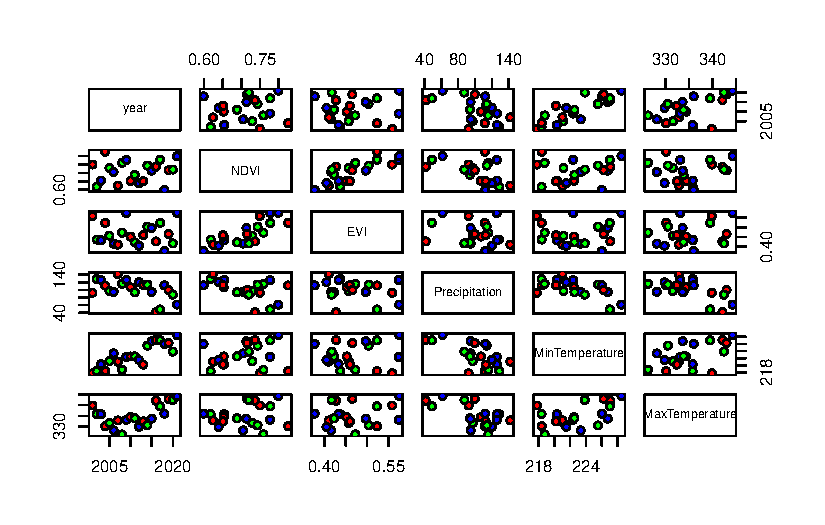
\includegraphics{Quarto_files/figure-pdf/fig-Pairs Plot-1.pdf}\{\#fig-Pairs
Plot fig-pos=`H'\}

\begin{Shaded}
\begin{Highlighting}[]
\FunctionTok{summary}\NormalTok{(}\FunctionTok{lm}\NormalTok{(EVI}\SpecialCharTok{\textasciitilde{}}\NormalTok{Precipitation}\SpecialCharTok{+}\NormalTok{MinTemperature}\SpecialCharTok{+}\NormalTok{MaxTemperature,Time\_Serie))}
\end{Highlighting}
\end{Shaded}

\begin{verbatim}

Call:
lm(formula = EVI ~ Precipitation + MinTemperature + MaxTemperature, 
    data = Time_Serie)

Residuals:
     Min       1Q   Median       3Q      Max 
-0.07335 -0.04589 -0.01146  0.03952  0.12389 

Coefficients:
                 Estimate Std. Error t value Pr(>|t|)
(Intercept)     0.8721110  1.5041062   0.580    0.570
Precipitation  -0.0006584  0.0007387  -0.891    0.385
MinTemperature -0.0031942  0.0053660  -0.595    0.560
MaxTemperature  0.0011142  0.0033124   0.336    0.741

Residual standard error: 0.05987 on 17 degrees of freedom
Multiple R-squared:  0.0783,    Adjusted R-squared:  -0.08436 
F-statistic: 0.4814 on 3 and 17 DF,  p-value: 0.6996
\end{verbatim}

::: \{\#tbl-Analysis of Variance Table .cell tbl-cap=`ANOVA Table for
Climate Date and Vegetation Loss In Ghana'\}

\begin{Shaded}
\begin{Highlighting}[]
\NormalTok{lm}\OtherTok{\textless{}{-}}\FunctionTok{lm}\NormalTok{(EVI}\SpecialCharTok{\textasciitilde{}}\NormalTok{ Precipitation }\SpecialCharTok{+}\NormalTok{ MinTemperature }\SpecialCharTok{+}\NormalTok{MaxTemperature,Time\_Serie)}
\FunctionTok{kable}\NormalTok{(}\FunctionTok{anova}\NormalTok{(lm),}\AttributeTok{booktab =}\NormalTok{ T) }\SpecialCharTok{\%\textgreater{}\%}
  \FunctionTok{kable\_styling}\NormalTok{(}\AttributeTok{latex\_options =} \FunctionTok{c}\NormalTok{(}\StringTok{"repeat\_header"}\NormalTok{))}
\end{Highlighting}
\end{Shaded}

\begin{table}
\centering
\begin{tabular}{lrrrrr}
\toprule
  & Df & Sum Sq & Mean Sq & F value & Pr(>F)\\
\midrule
Precipitation & 1 & 0.0037387 & 0.0037387 & 1.0430853 & 0.3214201\\
MinTemperature & 1 & 0.0010319 & 0.0010319 & 0.2878889 & 0.5985287\\
MaxTemperature & 1 & 0.0004055 & 0.0004055 & 0.1131364 & 0.7407174\\
Residuals & 17 & 0.0609334 & 0.0035843 & NA & NA\\
\bottomrule
\end{tabular}
\end{table}

:::

\hypertarget{non-parametric-analysis}{%
\subsection{Non-Parametric Analysis}\label{non-parametric-analysis}}

\hypertarget{time-series-analysis}{%
\subsection{\texorpdfstring{\textbf{Time-series
analysis}}{Time-series analysis}}\label{time-series-analysis}}

\hypertarget{steps-involved-in-box-jenkins-approach}{%
\subsubsection{\texorpdfstring{\uline{\textbf{Steps involved in
Box-Jenkins
approach}}}{Steps involved in Box-Jenkins approach}}\label{steps-involved-in-box-jenkins-approach}}

\begin{figure}

{\centering 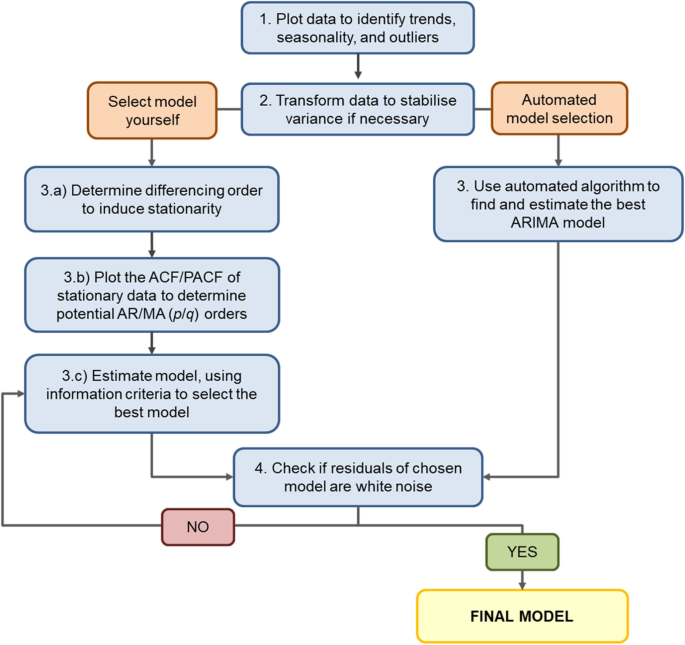
\includegraphics{Plots/Steps.png}

}

\caption{FlowChart}

\end{figure}

\hypertarget{chapter-four}{%
\chapter{CHAPTER FOUR}\label{chapter-four}}

\hypertarget{analysis-and-finding}{%
\subsection{Analysis and Finding}\label{analysis-and-finding}}

Before building an ARIMA model we checked that if the series is
stationary. That is, we needed to be determined that the time series is
constant in mean and variance are constant and not dependent on
time.Here, we look at a couple of methods for checking stationarity. If
the time series is provided with seasonarity, a trend, or a change point
in the mean or variance, then the influences need to be removed or
accounted for. Augmented Dickey--Fuller (ADF) t-statistic test to find
if the series has a unit root (a series with a trend line will have a
unit root and result in a large p-value).

\begin{Shaded}
\begin{Highlighting}[]
\CommentTok{\# The Stationary Signal and ACF}
\FunctionTok{plot}\NormalTok{(Rt,}\AttributeTok{col=} \StringTok{"red"}\NormalTok{, }\AttributeTok{main =} \StringTok{"Stationary Signal"}\NormalTok{)}
\FunctionTok{acf}\NormalTok{(Rt, }\AttributeTok{lag.max =} \FunctionTok{length}\NormalTok{(Rt),}
    \AttributeTok{xlab =} \StringTok{"lag"}\NormalTok{, }\AttributeTok{ylab =} \StringTok{\textquotesingle{}ACF\textquotesingle{}}\NormalTok{, }\AttributeTok{main =} \StringTok{\textquotesingle{}\textquotesingle{}}\NormalTok{)}

\CommentTok{\#The Trend Signal anf ACF}

\FunctionTok{plot}\NormalTok{(Tt,}\AttributeTok{col=} \StringTok{"red"}\NormalTok{,}\AttributeTok{main =} \StringTok{"Trend Signal"}\NormalTok{)}
\FunctionTok{acf}\NormalTok{(Tt, }\AttributeTok{lag.max =} \FunctionTok{length}\NormalTok{(Tt),}
    \AttributeTok{xlab =} \StringTok{"lag"}\NormalTok{, }\AttributeTok{ylab =} \StringTok{"ACF"}\NormalTok{, }\AttributeTok{main =} \StringTok{\textquotesingle{}\textquotesingle{}}\NormalTok{)}
\end{Highlighting}
\end{Shaded}

\begin{figure*}

\begin{minipage}[t]{0.50\linewidth}

{\centering 

\raisebox{-\height}{

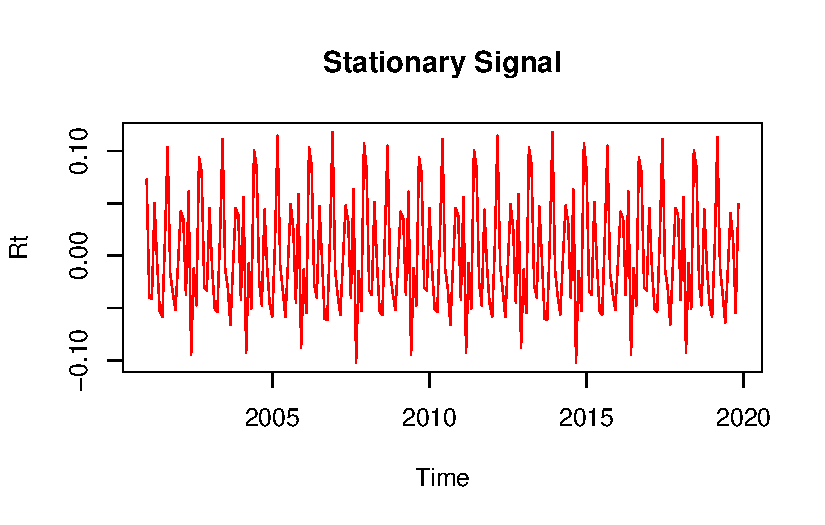
\includegraphics{Quarto_files/figure-pdf/fig-ACF-1.pdf}

}

}

\subcaption{\label{fig-ACF-1}Stationary Signal}
\end{minipage}%
%
\begin{minipage}[t]{0.50\linewidth}

{\centering 

\raisebox{-\height}{

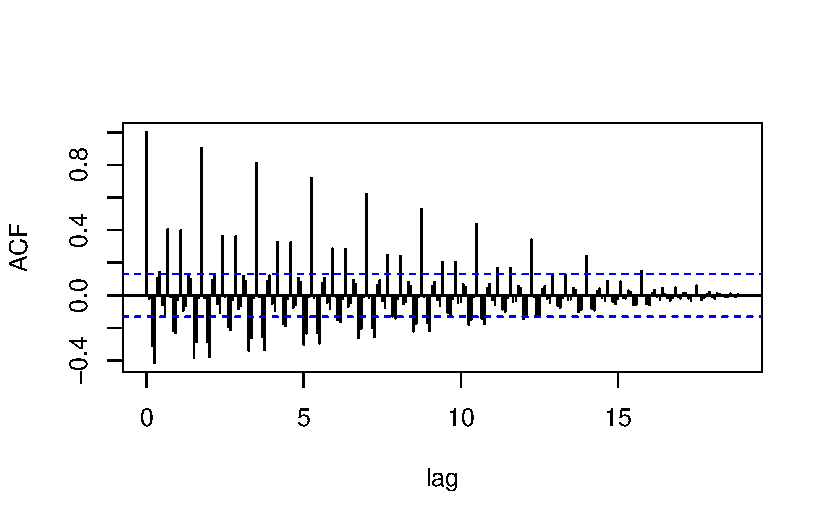
\includegraphics{Quarto_files/figure-pdf/fig-ACF-2.pdf}

}

}

\subcaption{\label{fig-ACF-2}Trend Signal}
\end{minipage}%
\newline
\begin{minipage}[t]{0.50\linewidth}

{\centering 

\raisebox{-\height}{

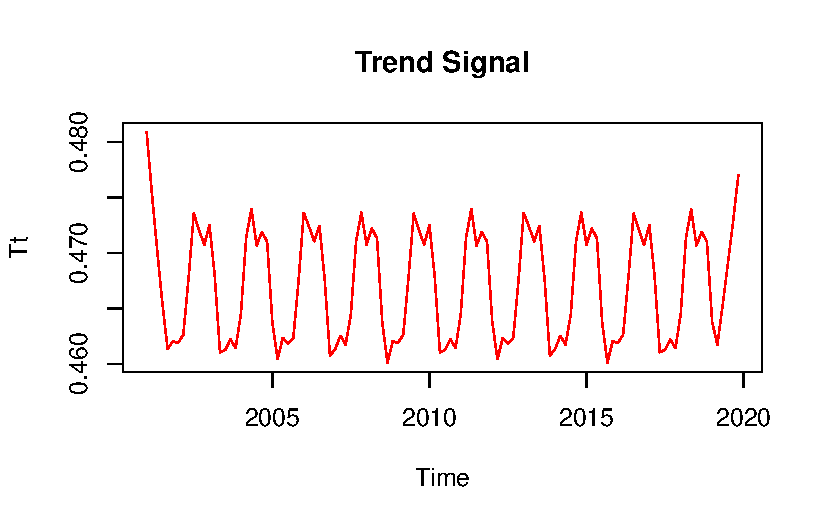
\includegraphics{Quarto_files/figure-pdf/fig-ACF-3.pdf}

}

}

\subcaption{\label{fig-ACF-3}Stationary Signal}
\end{minipage}%
%
\begin{minipage}[t]{0.50\linewidth}

{\centering 

\raisebox{-\height}{

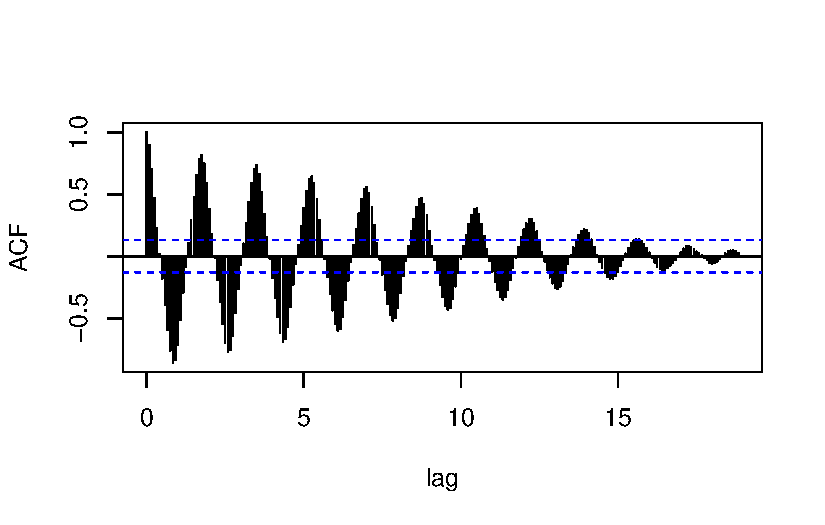
\includegraphics{Quarto_files/figure-pdf/fig-ACF-4.pdf}

}

}

\subcaption{\label{fig-ACF-4}Trend Signal}
\end{minipage}%

\caption{\label{fig-ACF}ACF Plot and PACF plot analysis for sample
between 2000 and 2020:}

\end{figure*}

\textbf{Discuss:}Shows the initial ACF plot and we can see that before
lag 25 almost all are significant and having no trend it needs to be
differentiated before performing any analysis. Clearly the seasonality
is visible even in the ACF plot.

\textbf{Dickey-Fuller Test and Plot}

\begin{Shaded}
\begin{Highlighting}[]
\NormalTok{tseries}\SpecialCharTok{::}\FunctionTok{adf.test}\NormalTok{(Tt)}
\end{Highlighting}
\end{Shaded}

\begin{verbatim}

    Augmented Dickey-Fuller Test

data:  Tt
Dickey-Fuller = -19.266, Lag order = 6, p-value = 0.01
alternative hypothesis: stationary
\end{verbatim}

\textbf{Discuss:}The DF test confirms that it is stationary as p value
\textless{} 0.05 and thus can be used for further analysis.This is after
doing double differentiation.It is noteworthy that the stationary signal
(top left) generates few significant lags that are larger than the ACF's
confidence interval (blue dotted line, bottom left). In contrast,
practically all delays in the time series with a trend (top right)
surpass the ACF's confidence range (bottom right). Qualitatively, we can
observe and infer from the ACFs that the signal on the left is steady
(due to the lags that die out) whereas the signal on the right is not
(since later lags exceed the confidence interval).

\hypertarget{specification-of-the-model}{%
\subsection{Specification of the
Model}\label{specification-of-the-model}}

We can create the SARMA model as SARMA(,0,)X(0)~based on the previous
study ~

If there hasn't been any differentiation, we can label it as zero. With
the first parameter being PACF and the second being ACF, the first
component of multiplication is the non-seasonal part.

The SARMA model's seasonal component follows a similar approach. Since
this model has a larger value than the prior SARMA model, it cannot be
used. We can utilize the GARCH model and test to see whether the AIC
value is better along with the ARMA model as well by omitting the
seasonal element as the seasonality pattern is not guaranteed.
Generalized Auto-Regressive Conditional Heteroskedasticity models, or
GARCH models, can be abbreviated. The GARCH model is commonly used, to
estimate value returns for stocks and other financial instruments where
trends are unknown. In order to~improved the~AIC values, we are testing
in our case study. Utilizing rugarch, we'll apply the seasonal
ARMA-GARCH model.\\
Since the data is stationary, we go about finding the p and q values
from ACF and PACF plots or use auto.arima() in R.

\begin{Shaded}
\begin{Highlighting}[]
\FunctionTok{auto.arima}\NormalTok{(Time\_Series)}
\end{Highlighting}
\end{Shaded}

\begin{verbatim}
Series: Time_Series 
ARIMA(3,0,0)(2,0,2)[12] with non-zero mean 

Coefficients:
          ar1      ar2      ar3    sar1     sar2     sma1     sma2    mean
      -0.1844  -0.4666  -0.2758  0.0626  -0.2229  -0.5593  -0.1545  0.4669
s.e.   0.0655   0.0739   0.0789  0.3384   0.1187   0.3338   0.2796  0.0004

sigma^2 = 0.001793:  log likelihood = 393.81
AIC=-769.62   AICc=-768.79   BIC=-738.8
\end{verbatim}

\textbf{Discuss:}As we are not differencing the model we can consider
ARMA(2,0,3) has the best model. Which is the best \emph{p} and \emph{q}
value also found from the ACF and PACF plots.

\textbf{Residual Analysis}

\textbf{Discuss:}From the above time series plot we can conclude that,
the trend within the year values for 1960,2016 and 2020 are similar. We
can observe that during start of the year in January the unemployment
rate increases and becomes constant during February, March and then
decreases sharply post April. Then in mid of the year it increases to a
certain level and attains constant until late/end of the year. Clearly
we can see some pattern when we do time series plot within a single
year. It can be concluded that unemployment rate is higher during winter
months and decreased post April which is summer season. Thus the
seasonal aspect can be clearly understood.\\

\hypertarget{modeling-and-parameter-estimation}{%
\subsection{\texorpdfstring{\textbf{Modeling and Parameter
estimation}}{Modeling and Parameter estimation}}\label{modeling-and-parameter-estimation}}

\hfill\break
Where the \textbf{ARIMA (PACF, Num\_Diffrentation, ACF)} model have the
below format for the parameters. Coefficients for various models:

\textbf{Discuss:}Based on the different models, we can see that
ARIMA(2,2,5) had the least AIC value, sigma\^{}2 being the least
therefore is the best model for given time series. Find the below time
series plot for the residuals.

\hypertarget{residual-analysis}{%
\subsubsection{\texorpdfstring{\textbf{Residual
Analysis}}{Residual Analysis}}\label{residual-analysis}}

\hypertarget{residual-plot}{%
\subsubsection{\texorpdfstring{\textbf{Residual
Plot}}{Residual Plot}}\label{residual-plot}}

\hypertarget{shapiro-test}{%
\subsubsection{\texorpdfstring{\textbf{Shapiro
Test}}{Shapiro Test}}\label{shapiro-test}}

\hypertarget{ljung-box}{%
\subsubsection{\texorpdfstring{\textbf{Ljung-Box}}{Ljung-Box}}\label{ljung-box}}

\textbf{Time-series Forecasting}

\textbf{Discuss:}The plot shows the forecasting to plot for the next 20
values which is shown by the blue region.

\begin{Shaded}
\begin{Highlighting}[]
\CommentTok{\#| tbl{-}cap: "Linear regression model for predicting EVI from Time"}
\NormalTok{tdx.ns }\OtherTok{\textless{}{-}} \FunctionTok{data.frame}\NormalTok{(}\AttributeTok{time =} \FunctionTok{c}\NormalTok{(}\DecValTok{1}\SpecialCharTok{:}\FunctionTok{length}\NormalTok{(Time\_Series)), }\AttributeTok{trend =}\NormalTok{ Time\_Series }\SpecialCharTok{{-}}\NormalTok{ tdx.dcp}\SpecialCharTok{$}\NormalTok{time.series[,}\DecValTok{1}\NormalTok{])}
\NormalTok{summary }\OtherTok{\textless{}{-}} \FunctionTok{summary}\NormalTok{(}\FunctionTok{lm}\NormalTok{(}\AttributeTok{formula =}\NormalTok{ trend }\SpecialCharTok{\textasciitilde{}}\NormalTok{ time, }\AttributeTok{data =}\NormalTok{ tdx.ns))}
\NormalTok{summary}
\end{Highlighting}
\end{Shaded}

\begin{table}

\caption{\textbf{?(caption)}}\begin{minipage}[t]{\linewidth}

{\centering 

\begin{verbatim}

Call:
lm(formula = trend ~ time, data = tdx.ns)

Residuals:
     Min       1Q   Median       3Q      Max 
-0.09840 -0.04340 -0.01218  0.04358  0.11309 

Coefficients:
             Estimate Std. Error t value Pr(>|t|)    
(Intercept) 4.668e-01  7.423e-03  62.888   <2e-16 ***
time        1.503e-06  5.645e-05   0.027    0.979    
---
Signif. codes:  0 '***' 0.001 '**' 0.01 '*' 0.05 '.' 0.1 ' ' 1

Residual standard error: 0.05574 on 225 degrees of freedom
Multiple R-squared:  3.151e-06, Adjusted R-squared:  -0.004441 
F-statistic: 0.000709 on 1 and 225 DF,  p-value: 0.9788
\end{verbatim}

}

\end{minipage}%

\end{table}

\begin{Shaded}
\begin{Highlighting}[]
\FunctionTok{plot}\NormalTok{(tdx.ns)}
\FunctionTok{abline}\NormalTok{(}\AttributeTok{a =}\NormalTok{ summary}\SpecialCharTok{$}\NormalTok{coefficients[}\DecValTok{1}\NormalTok{,}\DecValTok{1}\NormalTok{], }\AttributeTok{b =}\NormalTok{ summary}\SpecialCharTok{$}\NormalTok{coefficients[}\DecValTok{2}\NormalTok{,}\DecValTok{1}\NormalTok{], }\AttributeTok{col =} \StringTok{\textquotesingle{}blue\textquotesingle{}}\NormalTok{)}
\end{Highlighting}
\end{Shaded}

\begin{figure}[H]

{\centering 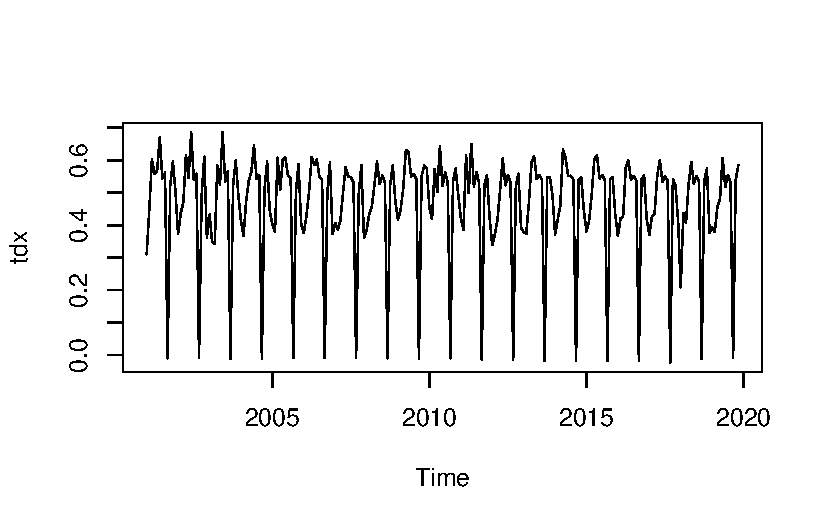
\includegraphics{Quarto_files/figure-pdf/unnamed-chunk-13-1.pdf}

}

\end{figure}

\begin{Shaded}
\begin{Highlighting}[]
\FunctionTok{plot}\NormalTok{(evi.hw }\OtherTok{\textless{}{-}}\NormalTok{ forecast}\SpecialCharTok{::}\FunctionTok{hw}\NormalTok{(}\AttributeTok{y =}\NormalTok{ Time\_Series, }\AttributeTok{h =} \DecValTok{12}\NormalTok{, }\AttributeTok{damped =}\NormalTok{ T))}
\end{Highlighting}
\end{Shaded}

\begin{figure}[H]

{\centering 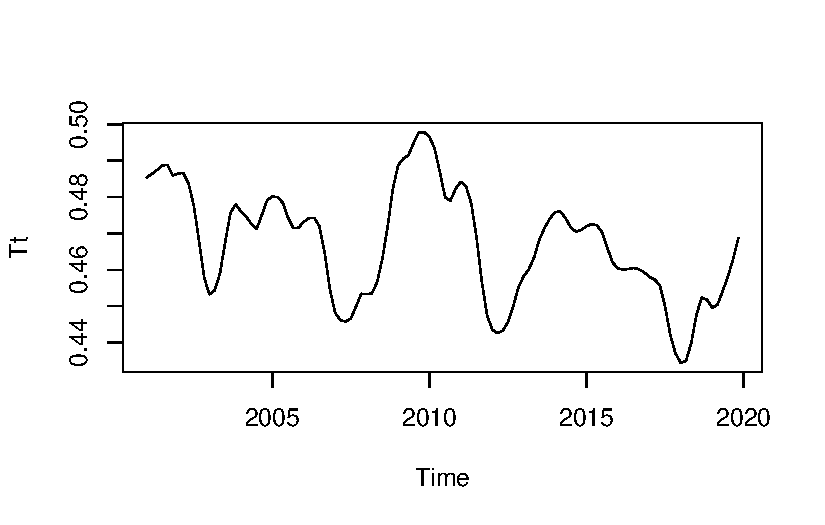
\includegraphics{Quarto_files/figure-pdf/unnamed-chunk-15-1.pdf}

}

\end{figure}

\hypertarget{chapter-five}{%
\chapter{CHAPTER FIVE}\label{chapter-five}}

\hypertarget{conclusions-and-recommendations}{%
\section{CONCLUSIONS AND
RECOMMENDATIONS}\label{conclusions-and-recommendations}}

\hypertarget{summary}{%
\subsection{Summary}\label{summary}}

Broadly speaking, in this study we have presented a state-of-the-art of
the following popular time series forecasting models with their salient
features:

\begin{itemize}
\tightlist
\item
  The Box-Jenkins or ARIMA models for linear time series forecasting.
\item
  Some non-linear stochastic models, such as NMA, ARCH.
\item
  SVM based forecasting models; LS-SVM and DLS-SVM.
\end{itemize}

\hypertarget{conclusions}{%
\subsection{Conclusions}\label{conclusions}}

It has been seen that, the proper selection of the model orders (in case
of ARIMA), the number of input, hidden, output and the constant
hyper-parameters (in case of SVM) is extremely crucial for successful
forecasting. We have discussed the two important functions. AIC and BIC,
which are frequently used for ARIMA model selection.

We have considered a few important performance measures for evaluating
the accuracy of forecasting models. It has been understood that for
obtaining a reasonable knowledge about the overall forecasting error,
more than one measure should be used in practice. The last chapter
contains the forecasting results of our experiments, performed on six
real time series datasets. Our satisfactory understanding about the
considered forecasting models and their successful implementation can be
observed form the five performance measures and the forecast diagrams,
we obtained for each of the six datasets. However in some cases,
significant deviation can be seen among the original observations and
our forecast values. In such cases, we can suggest that a suitable data
preprocessing, other than those we have used in our work may improve the
forecast performances.

\hypertarget{recommendations}{%
\subsection{Recommendations}\label{recommendations}}

Time series forecasting is a fast growing area of research and as such
provides many scope for future works. One of them is the Combining
Approach, i.e. to combine a number of different and dissimilar methods
to improve forecast accuracy. A lot of works have been done towards this
direction and various combining methods have been proposed in literature
{[}8, 14, 15, 16{]}. Together with other analysis in time series
forecasting, we have thought to find an efficient combining model, in
future if possible. With the aim of further studies in time series
modeling and forecasting

\hypertarget{references}{%
\chapter*{References}\label{references}}
\addcontentsline{toc}{chapter}{References}

\hypertarget{refs}{}
\begin{CSLReferences}{1}{0}
\leavevmode\vadjust pre{\hypertarget{ref-allotey2017}{}}%
Allotey, Godwin Akweiteh. 2017. {``Stop Galamsey in 3 Weeks or Face the
Law - Amewu.''} \emph{Ghana News}, March.
\url{http://citifmonline.com/2017/03/29/stop-galamsey-in-3-weeks-or-face-the-law-amewu/}.

\leavevmode\vadjust pre{\hypertarget{ref-ansah2017}{}}%
Ansah, Marian Efe. 2017. {``Galamsey, Pollution Destroying Water Bodies
in Ghana - Water Company.''} \emph{Ghana News}, March.
\url{http://www.leakxgh.com/2017/05/galamsey-pollution-destroying-water.html}.

\leavevmode\vadjust pre{\hypertarget{ref-barenblitt2021}{}}%
Barenblitt, Abigail, Amanda Payton, David Lagomasino, Lola Fatoyinbo,
Kofi Asare, Kenneth Aidoo, Hugo Pigott, et al. 2021. {``The Large
Footprint of Small-Scale Artisanal Gold Mining in Ghana.''}
\emph{Science of the Total Environment} 781 (August).
\url{https://doi.org/10.1016/j.scitotenv.2021.146644}.

\leavevmode\vadjust pre{\hypertarget{ref-confiden}{}}%
{``Confidence Intervals: An Empirical Investigation of the Series in the
m-Competition - ScienceDirect.''} n.d.
\url{https://www.sciencedirect.com/science/article/abs/pii/0169207087900458}.

\leavevmode\vadjust pre{\hypertarget{ref-defries2010}{}}%
DeFries, Ruth S., Thomas Rudel, Maria Uriarte, and Matthew Hansen. 2010.
{``Deforestation Driven by Urban Population Growth and Agricultural
Trade in the Twenty-First Century.''} \emph{Nature Geoscience} 3 (3):
178181.

\leavevmode\vadjust pre{\hypertarget{ref-gertler2016}{}}%
Gertler, Paul J., Orie Shelef, Catherine D. Wolfram, and Alan Fuchs.
2016. {``The Demand for Energy-Using Assets Among the World's Rising
Middle Classes.''} \emph{American Economic Review} 106 (6): 13661401.

\leavevmode\vadjust pre{\hypertarget{ref-goldgu2017}{}}%
{``Gold, Guns and China: Ghana's Fight to End Galamsey.''} 2017.
\emph{African Arguments}, May.
\url{https://africanarguments.org/2017/05/30/gold-guns-and-china-ghanas-fight-to-end-galamsey/}.

\leavevmode\vadjust pre{\hypertarget{ref-gracia2018}{}}%
Gracia, Zindzy. 2018. {``Causes and Effects of Galamsey in Ghana.''}
\emph{Yen.com.gh - Ghana News.}, January.
\url{https://yen.com.gh/104844-causes-effects-galamsey-ghana.html}.

\leavevmode\vadjust pre{\hypertarget{ref-gyekye}{}}%
Gyekye, Joyce. n.d. {``MD of Ghana Water Company Limited Says Fight
Against Galamsey Is Being Lost.''} \emph{Ghana Broadcasting
Corporation}. \url{http://www.gbcghana.com/1.11923484}.

\leavevmode\vadjust pre{\hypertarget{ref-hipel1994}{}}%
Hipel, Keith W., and A. Ian McLeod. 1994. \emph{Time Series Modelling of
Water Resources and Environmental Systems}. Elsevier.

\leavevmode\vadjust pre{\hypertarget{ref-library2015}{}}%
Library, Wiley Online, and Mohammad Valipour. 2015. {``Long-Term Runoff
Study Using SARIMA and ARIMA Models in the United States.''}
\emph{Meteorological Applications} 22 (3): 592--98.
\url{https://doi.org/10.1002/MET.1491}.

\leavevmode\vadjust pre{\hypertarget{ref-owusu-nimo2018}{}}%
Owusu-Nimo, F., J. Mantey, K. B. Nyarko, Eugene Appiah-Effah, and A.
Aubynn. 2018. {``Spatial Distribution Patterns of Illegal Artisanal
Small Scale Gold Mining (Galamsey) Operations in Ghana: A Focus on the
Western Region.''} \emph{Heliyon} 4 (2): e00534.
\url{https://doi.org/10.1016/j.heliyon.2018.e00534}.

\leavevmode\vadjust pre{\hypertarget{ref-specht2015}{}}%
Specht, Maria Joana, Severino Rodrigo Ribeiro Pinto, Ulysses Paulino
Albuquerque, Marcelo Tabarelli, and Felipe PL Melo. 2015. {``Burning
Biodiversity: Fuelwood Harvesting Causes Forest Degradation in
Human-Dominated Tropical Landscapes.''} \emph{Global Ecology and
Conservation} 3: 200209.

\leavevmode\vadjust pre{\hypertarget{ref-womendi2009}{}}%
{``Women Die in Ghana Mine Collapse.''} 2009, November.
\url{http://news.bbc.co.uk/2/hi/africa/8356343.stm}.

\leavevmode\vadjust pre{\hypertarget{ref-zhang1998}{}}%
Zhang, Guoqiang, B. Eddy Patuwo, and Michael Y. Hu. 1998. {``Forecasting
with Artificial Neural Networks:: The State of the Art.''}
\emph{International Journal of Forecasting} 14 (1): 35--62.
\url{https://doi.org/10.1016/S0169-2070(97)00044-7}.

\end{CSLReferences}


\backmatter

\end{document}
